% Cole Nielsen niels538@umn.edu
% EE 2002 Spring 2015
% Formal Lab Report 1

%----------------------------------------------------------------------------------------
%	PACKAGES AND DOCUMENT CONFIGURATIONS
%----------------------------------------------------------------------------------------

\documentclass[12pt]{article}

\usepackage{circuitikz}
\usepackage{graphicx}
\usepackage{subcaption}
\usepackage[top=1in, bottom= 1in, left=1in, right= 1in]{geometry}
\setlength\parindent{0pt}
\usepackage{fancyhdr}
\pagestyle{fancy}
\usepackage{textcomp}
\usepackage{tikz}
\usepackage{siunitx}
\usepackage{placeins}
\usepackage{titlesec}
\usepackage{cancel} 
\usepackage{tikz}
\usetikzlibrary{shapes.geometric, arrows}
\tikzstyle{box} = [rectangle, rounded corners, minimum width = 3cm, minimum height = 1cm, text centered, draw = black]
\tikzstyle{arrow} = [thick,->,>=stealth]
\usepackage{placeins}

\usepackage{listings}
\usepackage{color}

\definecolor{dkgreen}{rgb}{0,0.6,0}
\definecolor{gray}{rgb}{0.5,0.5,0.5}
\definecolor{mauve}{rgb}{0.58,0,0.82}

\lstset{frame=tb,
  language=C,
  aboveskip=3mm,
  belowskip=3mm,
  showstringspaces=false,
  columns=flexible,
  basicstyle={\small\ttfamily},
  numbers=none,
  numberstyle=\tiny\color{gray},
  keywordstyle=\color{blue},
  commentstyle=\color{dkgreen},
  stringstyle=\color{mauve},
  breaklines=true,
  breakatwhitespace=true,
  tabsize=3
}

%----------------------------------------------------------------------------------------
%	DOCUMENT INFORMATION
%----------------------------------------------------------------------------------------

\title{Lab 8 Report\\ \vspace{0.3 in} EE 4341}

\newcommand{\mymeter}[2]{   	% #1 = name , #2 = rotation angle
 \begin{scope}[transform shape,rotate=#2]
   \draw[thick] (#1)node(){$\mathbf V$} circle (11pt);
   \draw[rotate=45,-latex] (#1)  +(-17pt,0) --+(17pt,0);
 \end{scope}
}
\date{Spring 2016}
\begin{document}
\maketitle 
\begin{center}
 \begin{tabular}{l r}
   Cole \textsc{Nielsen} & niels538@umn.edu\\ 
\end{tabular}
\end{center}
\pagebreak
\pagebreak
%---------------------------------------------------------------------------------------
%----------------------------------------------------------------------------------------
%	Introduction
%----------------------------------------------------------------------------------------
\begin{abstract} 
\noindent A tic-tac-toe game was implemented using a PIC32 USB Starter Kit II and a 3.2 inch color touchscreen daughter board. The game implementation was performed using the Microchip graphical library in order to draw the graphical elements for the game, and a simple state machine controller was used to invoke the graphics updates in accordance to screen touch events.
\end{abstract}
\hrulefill
\section{Introduction}
The tic-tac-toe game was implemented by using the Microchip Graphics library on a PIC32 to drive a LCD display. The Microchip graphics library is a C library for PIC microcontrollers that has a whole family of functions capable of drawing shapes, text, images and widgets when used with a LCD and controller. The library supports both primitive functions and graphical objects. The primitive functions directly create graphics on the display that can only be changed by redrawing the whole screen. Graphical objects add a layer of abstraction by treating every graphic on the screen as a object, like a sort of "variable" that can be changed at anytime without affecting other graphics on the screen. Every graphical object has a set of variables associated with it in a struct that describes things such as color, location and status, of which can be changed by a function to update the object on the display. Treating the graphics as objects also has benefits beyond being able to change a single object on the screen without affecting others, it makes it easier to keep track of graphics as they all are assigned an ID. For the implementation in this lab, graphical objects were predominantly used to build the graphical interface, with BUTTON objects constituting the tic-tac-toe grid. A simple control state machine was then coded to update the displayed objects according to the display presses and the rules of tic-tac-toe.
\section{Implementation}
The Tic-Tac-Toe game was implemented in two parts, an initial part used to configure the screen and all the objects, and then a control function that was used to update the graphical objects in accordance to sensed screen presses.
\subsection*{Initialization}
Using the given main file and the graphical library, which implemented all the necessary graphics (including the X and O images), the only thing that needed to be implemented for the intitialization phase was creating the display objects and primitives for the game, as well as other requisite declerations. Below is the code used for the tic-tac-toe graphics initialization:
\begin{lstlisting}
/////////////////////////////////////////////////////////////////////////////
//                          GLOBAL VARIABLES
/////////////////////////////////////////////////////////////////////////////

volatile DWORD      tick = 0;                           // tick counter
volatile int press[9]; //keeps track of plays
volatile XCHAR win[] = {'W','i','n','s',0};
volatile XCHAR lose[] = {'L','o','s','e','s',0};
volatile XCHAR draw[] = {'D','r','a','w',0};
volatile XCHAR Str[] = {'R','e','s','e','t',0};
volatile XCHAR turn[] = {'T','u','r','n',0};

/////////////////////////////////////////////////////////////////////////////
//                                  MAIN
/////////////////////////////////////////////////////////////////////////////

int main(void)
{
    int j;
    for (j = 0; j<9; j++) press[j]=0; //clears play array

    GOL_MSG msg; // GOL message structure to interact with GOL

        GOL_SCHEME* rScheme; // reset button scheme
        rScheme = GOLCreateScheme(); // Create alternative style

        // scheme
        rScheme->TextColor0 = WHITE; // set text color 0
        rScheme->TextColor1 = WHITE; // set text color 1
        rScheme->Color0 = BLUE; // set text color 0
        rScheme->Color1 = BLUE; // set text color 1
        rScheme->EmbossDkColor = BLUE;     // Emboss dark color used for 3d effect.
        rScheme->EmbossLtColor = BLUE;
        GOL_SCHEME* gridScheme; // tic tac toe grid button scheme

        gridScheme = GOLCreateScheme(); // Create alternative style

        // scheme
        gridScheme->TextColor0 = BLACK; // set text color 0
        gridScheme->TextColor1 = BLACK; // set text color 1
        gridScheme->Color0 = WHITE; // set text color 0
        gridScheme->Color1 = WHITE; // set text color 1
        gridScheme->EmbossDkColor = WHITE;     // Emboss dark color used for 3d effect.
        gridScheme->EmbossLtColor = WHITE;
        
   	InitializeBoard(); //Initialize everything for the display

	SetColor(WHITE);

	ClearDevice();

        SetColor(BLACK);
        while(!Bar(78, 0, 82, GetMaxY()));
        while(!Bar(158, 0, 162, GetMaxY()));
        while(!Bar(0, 78, 240, 82));
        while(!Bar(0, 158, 240, 162));

        BtnCreate(  10, // reset
			        240, 200, GetMaxX(), GetMaxY(), // Object's dimension
			        NULL,
			        BTN_DRAW, // set state of the object:
			        // draw the object
			        NULL, // no bitmap used
			        Str, // use this text
			        rScheme);

        BtnCreate(  11, // turn text
			        240, 0, GetMaxX(), 39, // Object's dimension
			        NULL,
        			BTN_DRAW, // set state of the object:
			        // draw the object
			        NULL, // no bitmap used
			        turn, // use this text
			        gridScheme);

        BtnCreate(  12, // turn display
			        240, 40, GetMaxX(), 100, // Object's dimension
			        NULL,
			        BTN_DRAW, // set state of the object
			        // draw the object
			        &TTTX, // no bitmap used
			        NULL, // use this text
			        gridScheme);

        BtnCreate(  13, // win /lose/draw button
			        240, 101, GetMaxX(), 140, // Object's dimension
			        NULL,
			        BTN_DRAW, // set state of the object:
			        // draw the object
			        NULL, // no bitmap used
			        NULL, // use this text
			        gridScheme);



        BtnCreate(  1, // 1st Button ID
                    0, 0, 77, 77,NULL, // Object's dimension
                    BTN_DRAW, // set state of the object:
                    // draw the object
                    NULL, // no bitmap used
                    NULL, // use this text
                    gridScheme);

        BtnCreate(  2, //
                    82, 0, 157, 77,NULL, // Object's dimension
                    BTN_DRAW, // set state of the object:
                    // draw the object
                    NULL, // no bitmap used
                    NULL, // use this text
                    gridScheme);

        BtnCreate(  3, // 
                    162, 0, 239, 77,NULL, // Object's dimension
                    BTN_DRAW, // set state of the object:
                    // draw the object
                    NULL, // no bitmap used
                    NULL, // use this text
                    gridScheme);

        BtnCreate(  4, // 
                    0, 82, 77, 157,NULL, // Object's dimension
                    BTN_DRAW, // set state of the object:
                    // draw the object
                    NULL, // no bitmap used
                    NULL, // use this text
                    gridScheme);

        BtnCreate(  5, // 
                    82, 82, 157, 157,NULL, // Object's dimension
                    BTN_DRAW, // set state of the object
                    // draw the object
                    NULL, // no bitmap used
                    NULL, // use this text
                    gridScheme);

        BtnCreate(  6, // 
                    162, 82, 239, 157,NULL, // Object's dimension
                    BTN_DRAW, // set state of the object:
                    // draw the object
                    NULL, // no bitmap used
                    NULL, // use this text
                    gridScheme);

        BtnCreate(  7, // 
                    0, 162, 77, GetMaxY(),NULL, // Object's dimension
                    BTN_DRAW, // set state of the object:
                    // draw the object
                    NULL, // no bitmap used
                    NULL, // use this text
                    gridScheme);

        BtnCreate(  8, // 
                    82, 162, 157, GetMaxY(),NULL, // Object's dimension
                    BTN_DRAW, // set state of the object:
                    // draw the object
                    NULL, // no bitmap used
                    NULL, // use this text
                    gridScheme);

        BtnCreate(  9, //
                    162, 162, 239, GetMaxY(),NULL, // Object's dimension
                    BTN_DRAW, // set state of the object:
                    // draw the object
                    NULL, // no bitmap used
                    NULL, // use this text
                    gridScheme);
\end{lstlisting}
The first chunk of code is global variable intialization. A couple character strings are created so they can be displayed using the graphical objects, for scenarios like win or draw. Another array, press[] was also created with 9 elements to keep track of the key presses of each of the tic tac toe grid cells. The tracking scheme devised is that an unused cell has 0 in its corresponding array element, 1 for an X and 2 for a O. Moving on to the main function. Initially, the press tracking array is cleared to be all zeros, meaning that the board is clear upon start up. Then, a  message variable is created that is used for communication between the object functions for when events like a key press occur.Then, two color schemes for the graphical object layer (GOL) where created, used to set things like text, accent and background color. Two schemes were made, one (gridScheme) with everything white except for text, used for the tic tac toe grid buttons and text, and then one (rScheme) set to have white text with blue background for the reset button. For every button made, a scheme must be specified to set the coloring. The next part of the code uses several primitives to clear the LCD to white and to draw a tic tac toe grid. This is done by setting the draw color with SetColor(), and then calling primitive functions. The primitive functions used are ClearScreen(), to draw the whole screen one color, and then Bar() to draw a rectange with specfied side coordinates. In this case four bars where drawn in black for the grid. The last chunk of code are the object declerations. Objects in this library are created as structures that contain all the details pertaining to the object, such as color, state, physical location and so on. Only the BUTTON structure was used for this lab, to create squares that can either be colored, contain text, or a picture, or all three at once. Every object is given an ID (the first argument of the decleration), which is used in the future to modify the object. For this implementation, a total of thirteen buttons were created, nine (IDs 1-9) for the tic tac toe grid cells, one for the reset button (ID = 10), one for a text label saying "Turn" (ID = 11), one for an indicator showing whose turn it is (ID = 12) and another text button used to tell the players who won (ID=13). The tic tac toe grid buttons were assigned ID numbers like a standard number pad, with their physical location being in the left three quarters of the LCD (inhabiting a square). All the tic tac toe cells initially were set to show no graphic (empty). The right quarter of the screen was configured to have the reset button, the turn text, the player indicator (initially X) and a blank win indicator. 
\section{State controller for Tic-Tac-Toe}
The actual game play control was implemented in a sort of state machine that perpetually checked for presses on the screen, figured out what object those presses corresponded to, and then updated the LCD accordingly per the rules of tic-tac-toe. This functionality was implemented using a number of functions, which will be discussed in the following:
\begin{lstlisting}
        while(1){

              if(GOLDraw()){
                  TouchGetMsg(&msg);
                  GOLMsg(&msg);
              }
        }
}
\end{lstlisting}
This part of the code is at the end of the main fucntion. It is a infinite loop that perpetually updates the LCD using a library function GOLDraw() (graphical object layer draw), checks for touch screen events using TouchGetMsg(). TouchGetMsg() relays the touch screen event data to the GOL message variable msg, which is then processed by GOLMsg(). GOLMsg() decodes the touch screen data, deciphering the object corresponding to the display presses, and runs a function GOLMsgCallback(), which updates the objects according to those presses. The GOLMsgCallback() is shown below:
\begin{lstlisting}
WORD GOLMsgCallback(WORD objMsg, OBJ_HEADER *pObj, GOL_MSG *pMsg)
{
       WORD objectID;
       BUTTON *buttonObj;
       STATICTEXT *stObj;

       int i;
       int state = 0;

       for(i = 0; i<9; i++){
           if (press[i] != 0)
               state ^= 1;
       }
       
       buttonObj = (BUTTON*)GOLFindObject(12);
       
       if(state == 0)
            BtnSetBitmap(buttonObj, &TTTX);
       else BtnSetBitmap(buttonObj, &TTTO);

       objectID = GetObjID(pObj);
       if(objectID == 10){
           if (objMsg == BTN_MSG_PRESSED){
               for(i = 1; i<10; i++){
                  buttonObj = (BUTTON*)GOLFindObject(i);
                  BtnSetBitmap(buttonObj, NULL);
               }
                  for (i = 0; i<9; i++) press[i]=0;
           }
       }
       if(objectID<=9){
           if (objMsg == BTN_MSG_PRESSED){
                if((state == 0)&(press[objectID-1]==0)){
                    press[objectID-1]=1;
                    BtnSetBitmap(pObj, &TTTX);
                }
                else if((press[objectID-1]==0)){
                    press[objectID-1]=2;
                    BtnSetBitmap(pObj, &TTTO);
                }
           }
       }

       if((press[0]==press[1])&(press[1]==press[2])&(press[0]!=0)){
           if(state == 0){
               stObj = (STATICTEXT*)GOLFindObject(13);
               StSetText(stObj, win);
           }
       }
       
	return(1);
}
\end{lstlisting}
The GOLMsgCallback() takes three arguments provided by the GOLMsg() based on the touch data. For this implementation, only the argument pertaining to the touch event object *pObj is used. *pObj gives the value of the object pointed by the object pointer. This value is decoded into the according object ID using the GetObjID() function, which finds the object in the linked list holding all objects and extracts the ID. Before any operations are performed based upon that data, a statefinding operation is first performed, where state represents whose turn it currently is. The state is found by looping through the press[] array to see how many turns have been performed. For even or 0 turns, the state is set to 0 which corresponds to X's turn. For odd number of turns the state is set to one, which corresponds to O's turn. The turn indicator object (ID = 12) is also updated by finding its location in memory using GOLFindObject(), and storing it to a pointer for a BUTTON type. Using this pointer value, the function (almost like a class function) BtnSetBitmap() is used to set the turn indicator to an X or O depending on the current state. Next, the response to the touch screen event is determined, using a number of conditional statements. The first one checks to see if the ID corresponding to the touch event is 10, meaning the RESET button. If it is the reset button, the object message is checked to see if it corresponds to a button press, meaning a request for reset. If the button was pressed, a for loop is used to cycle through all the tic-tac-toe grid cells and reset them to be blank. The press[] array, used for keeping track of the moves is also reset to be corresponding to a blank grid (all zeros). The next conditional statement is used to check if the button pressed is of ID equal or less than 9, which corresponds to a button on the tic-tac-toe grid. If so, it is verified if the button was pressed using the object message, the grid cell will be filled with that turn's players symbol if that cell has not already been filled (done by checking that cell is equal to zero, which means blank).  All other buttons are ignored for key presses, that is there are no statments to check and update them according to keypresses in this function. The last chunk of code is used to check for a win. Note, this function is incomplete. The win checking was implemented by using if statements to check if all the elements in any three consecutive cells (vertical, horizontal or diagonal) are all equal and non zero. If this is the case, then the player who just made that move that is being evaluated by the win checking code has won, and accordingly the text win indicator is updated to say "Win" using StSetText(). The full win/draw detection code was not implemented due to time constraints. The full win checking code could be fully implemented by adding variants of the one win checking statement to check for all other winning combinations. Draw detection could be implemented by sensing when the press[] array is full, checking for any wins, and then if there are no wins then display "Draw".
\section{Summary}
The outcome of this lab was a partially functioning tic-tac-toe game built using a PIC32 with a LCD daughter board. The knowledge gained from this lab is valuable in that it can be used to develop graphical interfaces in future projects to interact with hardware. A major difficulty not overcome in the time alotted for this lab was getting the object update functionality to fully work. This was a problem in the GOLMsgCallback() function used to update objects according to touch screen events. In particular, the problem was that GOLFindObject() never worked for some instances, such as a for returning the pointer for a literal ID number argument, which made it impossible to reset the grid cells after a reset. It also prohibited the "win" text button to be updated to show when a player won, or if there was a draw. Overall, this limited the code only to being able to display the initial buttons and primitives, and then updates for the buttons on the grid. Below is an image showing the extent that the written code functioned:

\FloatBarrier
\begin{figure}[h!]
\begin{center}
 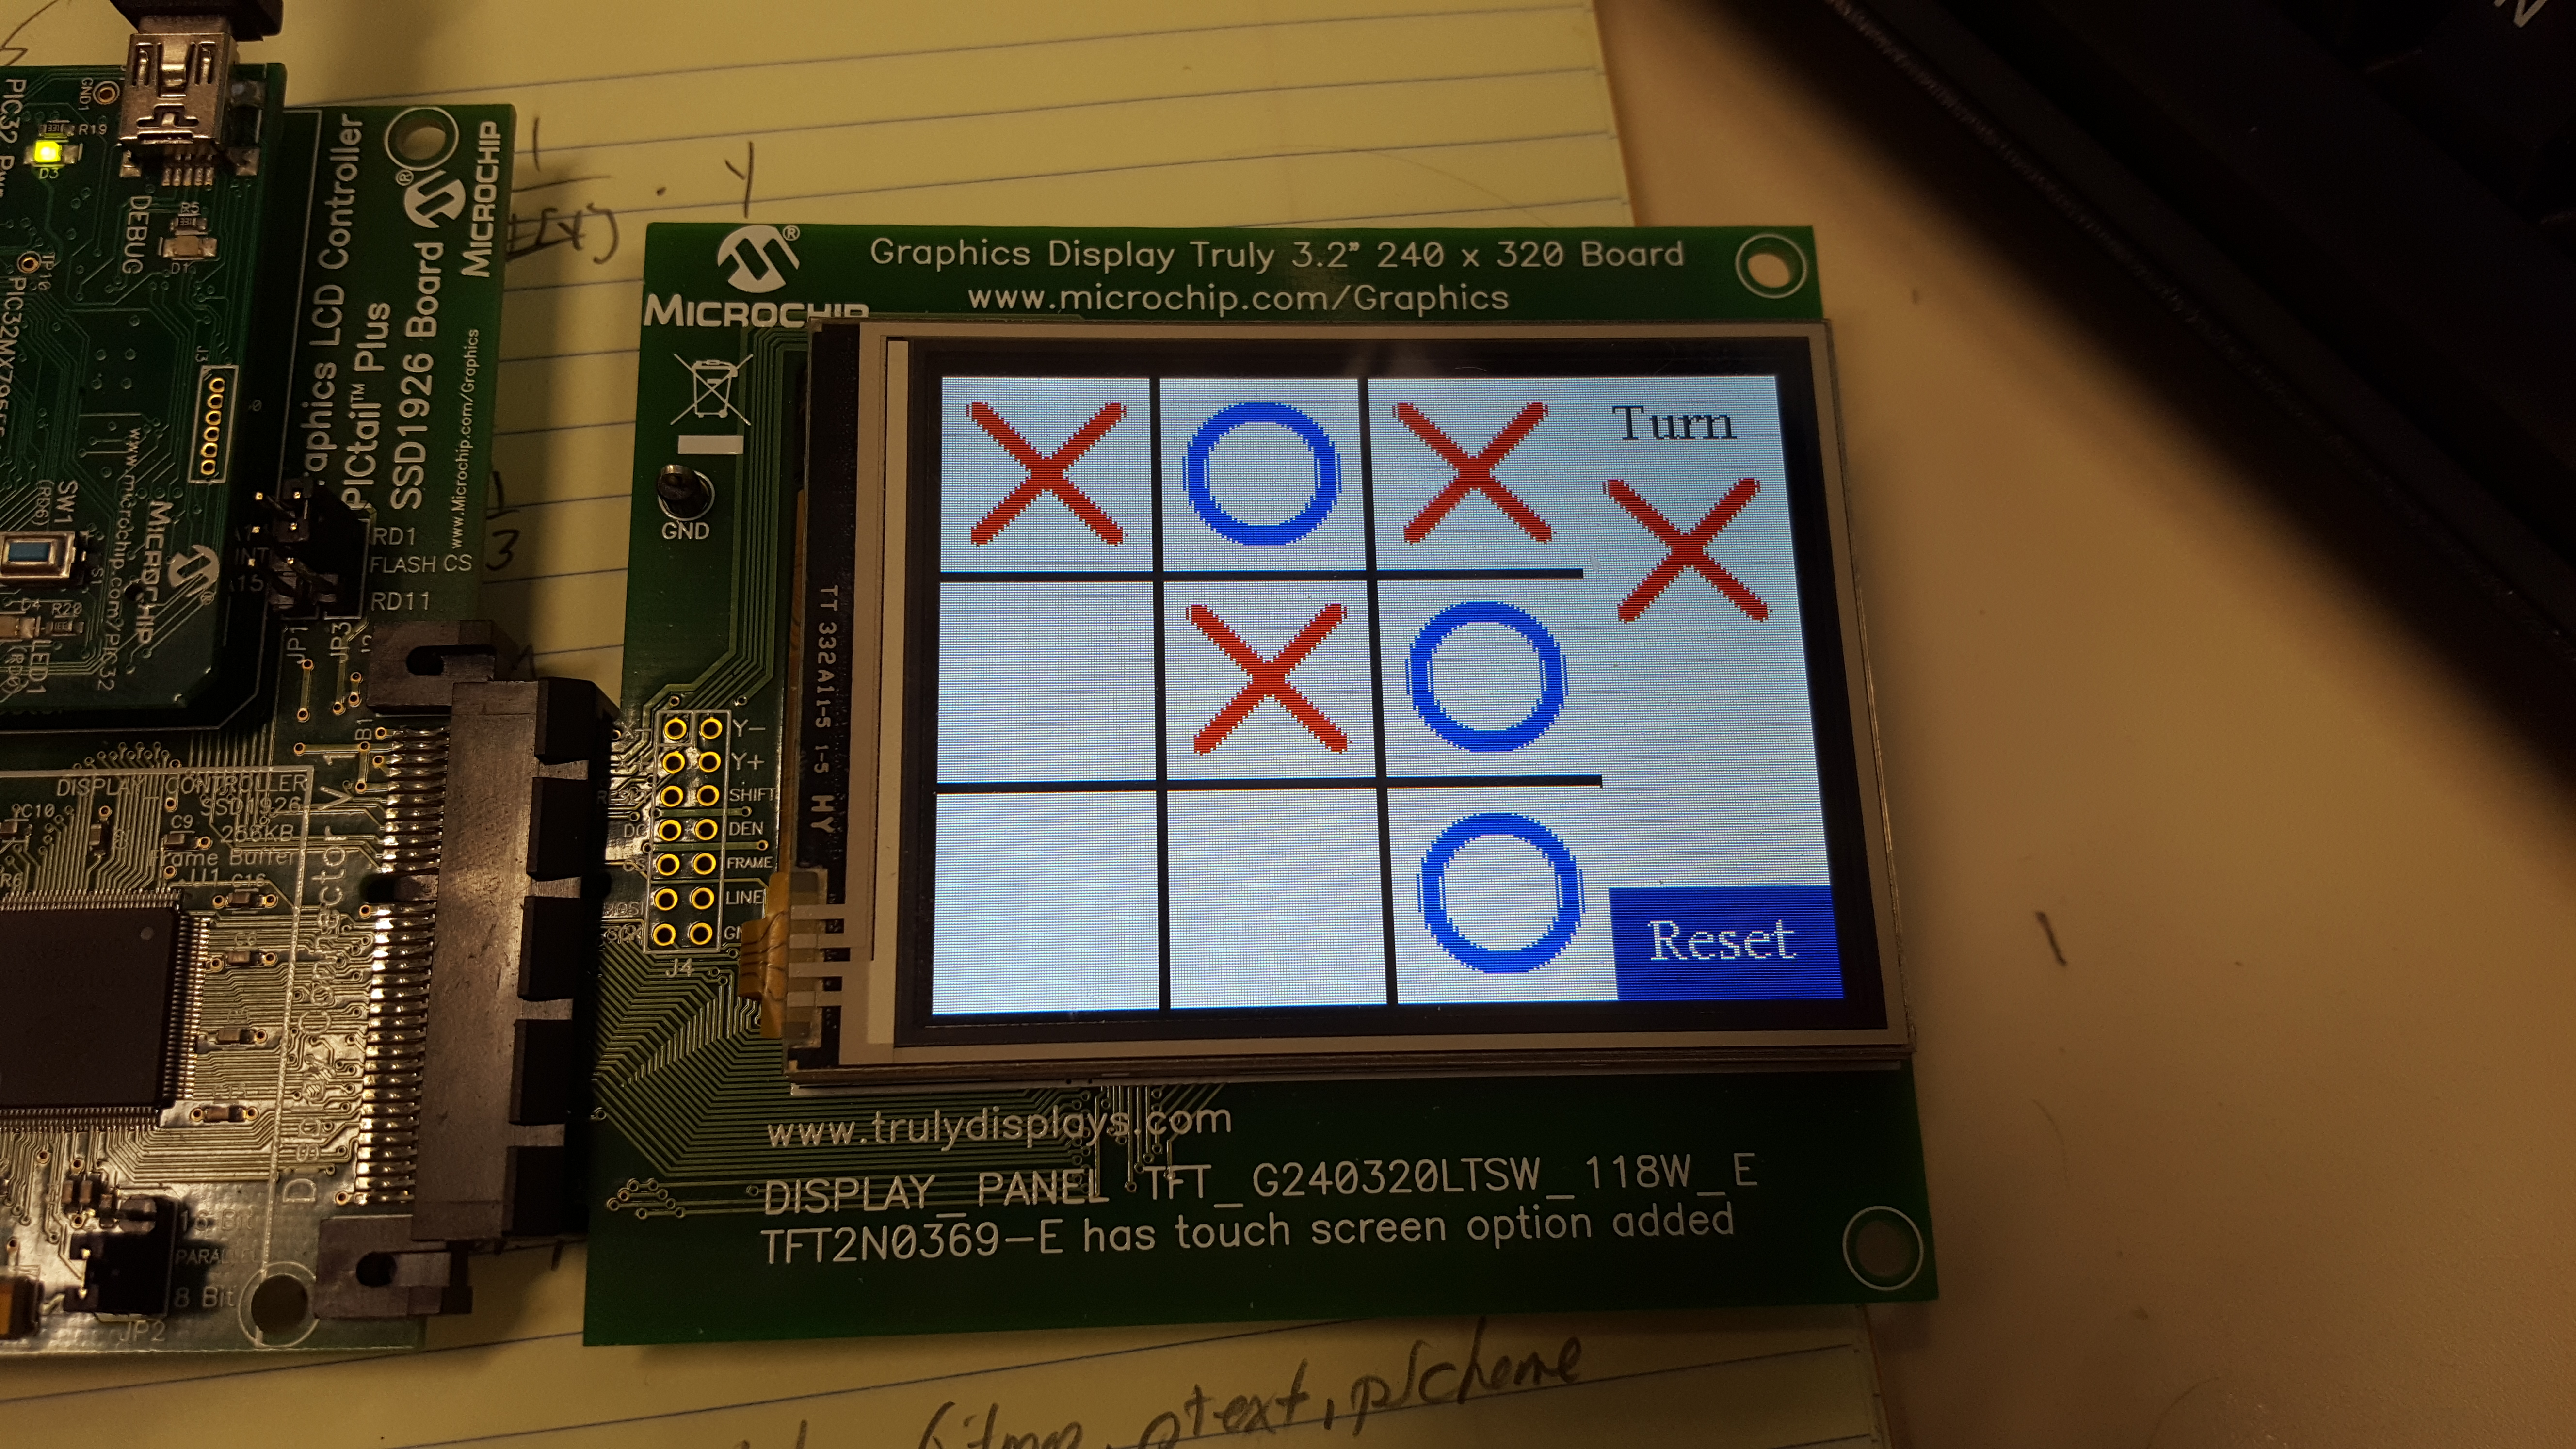
\includegraphics[scale=0.07]{./ex.jpg}
\end{center}
\end{figure}
\FloatBarrier
\end{document}
